\chapter{Complexvorming}\label{ch:b1:complexation}

Giet een beetje ammoniakoplossing in lichtblauw koper(II)sulfaat: er
ontstaat meteen een lichtblauw neerslag. Giet er meer bij, en het
neerslag lost op tot een oplossing met een diep, bijna inktachtig blauw.
Niets in de hoofdstukken over zuren en basen of over neerslagvorming
verklaart die tweede stap. De ammoniakmoleculen hebben zich via hun \omterm{def:b1:lewis-resonance-vsepr:lewis}{vrije
elektronenparen} aan het koperion gebonden en een nieuw deeltje gevormd,
een \omterm{def:b1:complexation:complex}{complex}, stabieler dan het hydroxide en met een andere kleur.
\omterm{def:b1:complexation:complex}{Complexen} vervoeren zuurstof in het bloed, houden het metaal vast in
chlorofyl en in vitamine B$_{12}$, maken hard water zachter en lossen
metalen op die met niets anders oplossen. Dit hoofdstuk behandelt ze als
nog een uitwisseling van deeltjes in water, met eigen constanten en
diagrammen.

\begin{recall}
\omterm{def:b1:lewis-resonance-vsepr:lewis-acid}{Lewiszuren} (acceptoren van elektronenparen), \omterm{def:b1:lewis-resonance-vsepr:lewis-acid}{lewisbasen} (donoren van
elektronenparen) en de \omterm{def:b1:lewis-resonance-vsepr:lewis-acid}{datieve binding} werden gedefinieerd in
\cref{ch:b1:lewis-resonance-vsepr}. De \omterm{def:b1:predominant-reaction:predominance}{predominantiediagrammen} en de
methode van de \omterm{def:b1:predominant-reaction:predominant-reaction}{predominante reactie} komen uit
\cref{ch:b1:predominant-reaction}; het \omterm{def:b1:precipitation:solubility-product}{oplosbaarheidsproduct} en de
voorwaarde voor neerslagvorming uit \cref{ch:b1:precipitation}.
\end{recall}

\begin{omfigure}
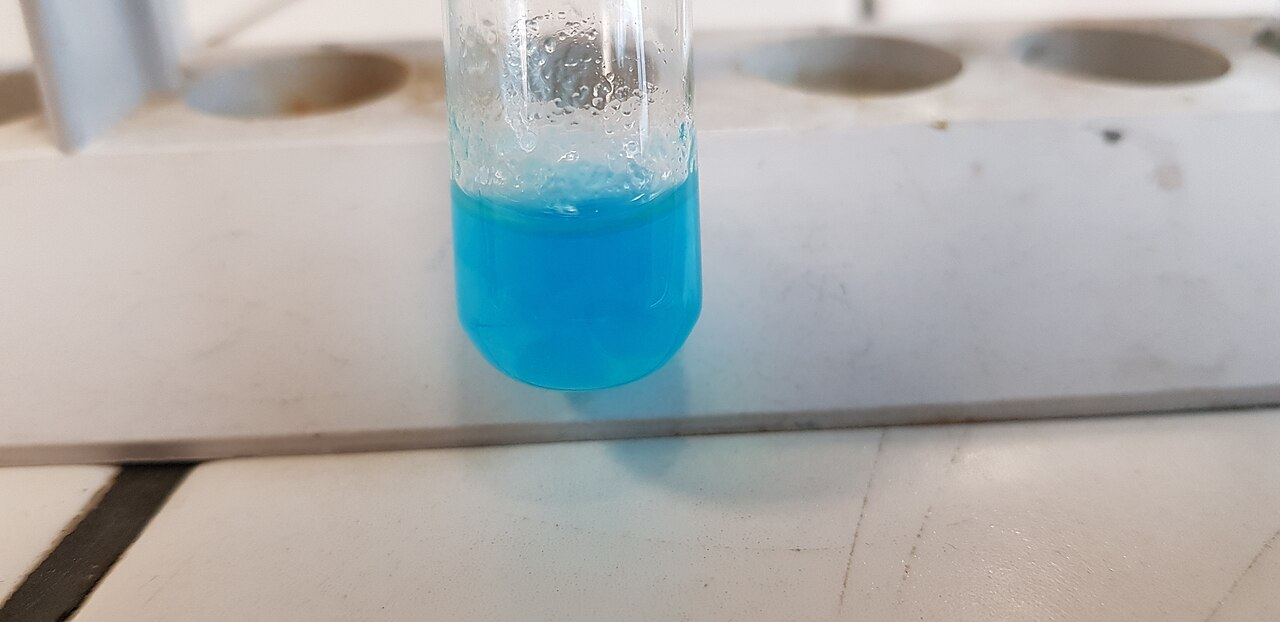
\includegraphics[height=4.2cm]{images/book2/copper-hydroxide.jpg}\hspace{0.6em}%
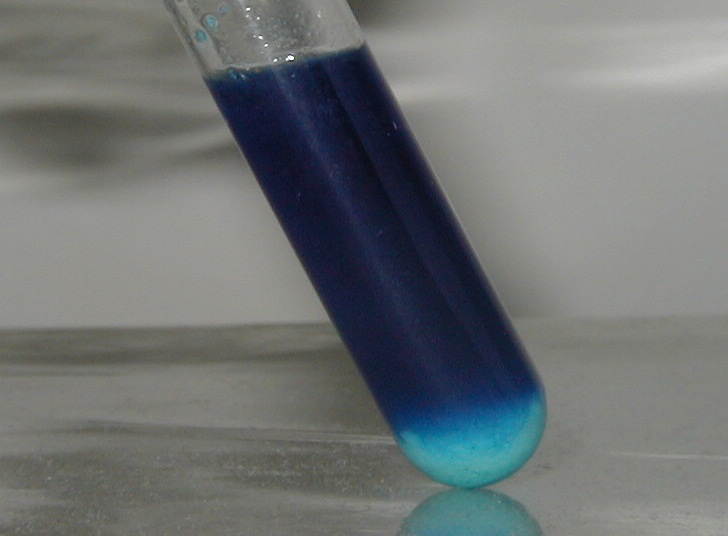
\includegraphics[height=4.2cm]{images/book2/copper-ammine.jpg}

{\small Links: een suspensie van lichtblauw koper(II)hydroxide
(foto Alvy16, CC BY 4.0). Rechts: met meer ammoniak lost de vaste stof op
tot het diepblauwe tetraamminekoper(II)ion; onderin de buis ligt nog wat
onopgelost hydroxide (foto Chemicalinterest, publiek domein). Beide
Wikimedia Commons.}
\end{omfigure}

\section{Complexen en liganden}

\begin{definition}[Complex, centraal atoom, ligand]\label{def:b1:complexation:complex}
Een \emph{complex}\index{complex} is een deeltje dat bestaat uit een
\emph{centraal atoom}\index{centraal atoom} of ion, meestal een
metaalkation dat als \omterm{def:b1:lewis-resonance-vsepr:lewis-acid}{lewiszuur} optreedt, dat via \omterm{def:b1:lewis-resonance-vsepr:lewis-acid}{datieve bindingen}
gebonden is aan moleculen of ionen die als \omterm{def:b1:lewis-resonance-vsepr:lewis-acid}{lewisbasen} optreden, de
\emph{liganden}\index{ligand}. Zijn formule wordt tussen vierkante haken
geschreven, met zijn totale lading: $[\ce{Cu(NH3)4}]^{2+}$,
$[\ce{Fe(CN)6}]^{4-}$, $[\ce{Ag(NH3)2}]^{+}$, $[\ce{FeSCN}]^{2+}$.
\end{definition}

De lading van het \omterm{def:b1:complexation:complex}{complex} is de som van de ladingen van het centrale ion
en van de \omterm{def:b1:complexation:complex}{liganden}: $\mathrm{Fe^{2+}}$ en zes \ce{CN-} geven
$[\ce{Fe(CN)6}]^{4-}$. Een \omterm{def:b1:complexation:complex}{ligand} heeft minstens één \omterm{def:b1:lewis-resonance-vsepr:lewis}{vrij elektronenpaar}
nodig: \ce{NH3}, \ce{H2O}, \ce{OH-}, \ce{Cl-}, \ce{CN-}, \ce{SCN-}
(gebonden via S of N). Elk metaalion in water is in feite al een \omterm{def:b1:complexation:complex}{complex}
met watermoleculen als \omterm{def:b1:complexation:complex}{liganden}, $[\ce{Cu(H2O)6}]^{2+}$ of
$[\ce{Fe(H2O)6}]^{3+}$; een ander \omterm{def:b1:complexation:complex}{complex} vormen betekent die
watermoleculen uitwisselen tegen andere \omterm{def:b1:complexation:complex}{liganden}, en de waterliganden
worden in de formules weggelaten, zoals \ce{H3O+} geschreven wordt voor
het gehydrateerde proton.

\begin{omfigure}
\begin{tikzpicture}[font=\small, line cap=round]
  % [Ag(NH3)2]+ : linear
  \begin{scope}
    \node (ag) at (0,0) {\ce{Ag}};
    \node (n1) at (-1.2,0) {\ce{H3N}};
    \node (n2) at (1.2,0) {\ce{NH3}};
    \draw[thick] (n1) -- (ag) -- (n2);
    \node at (0,-1.75) {$[\ce{Ag(NH3)2}]^{+}$, lineair};
  \end{scope}
  % [Cu(NH3)4]2+ : square plane in perspective
  \begin{scope}[xshift=4.3cm, every node/.style={fill=white, inner sep=1.5pt}]
    \node (cu) at (0,0) {\ce{Cu}};
    \node (a) at (-1.45,-0.5) {\ce{H3N}};
    \node (b) at (1.45,0.5) {\ce{NH3}};
    \node (c) at (0.85,-0.9) {\ce{NH3}};
    \node (d) at (-0.85,0.9) {\ce{H3N}};
    \begin{pgfonlayer}{background}
    \draw[gray, dashed] (a.center) -- (c.center) -- (b.center) -- (d.center) -- cycle;
    \end{pgfonlayer}
    \draw[thick] (cu) -- (a); \draw[thick] (cu) -- (b);
    \draw[thick] (cu) -- (c); \draw[thick] (cu) -- (d);
    \node at (0,-1.75) {$[\ce{Cu(NH3)4}]^{2+}$, vierkant vlak};
  \end{scope}
  % [Fe(CN)6]4- : octahedron
  \begin{scope}[xshift=9.2cm, every node/.style={fill=white, inner sep=1.5pt}]
    \node (fe) at (0,0) {\ce{Fe}};
    \node (t) at (0,1.3) {\ce{CN}};
    \node (u) at (0,-1.3) {\ce{CN}};
    \node (l) at (-1.45,-0.45) {\ce{NC}};
    \node (r) at (1.45,0.45) {\ce{CN}};
    \node (f) at (0.8,-0.8) {\ce{CN}};
    \node (k) at (-0.8,0.8) {\ce{NC}};
    \begin{pgfonlayer}{background}
    \draw[gray, dashed] (l.center) -- (f.center) -- (r.center) -- (k.center) -- cycle;
    \end{pgfonlayer}
    \foreach \x in {t,u,l,r,f,k} \draw[thick] (fe) -- (\x);
    \node at (0,-1.75) {$[\ce{Fe(CN)6}]^{4-}$, octaëdrisch};
  \end{scope}
\end{tikzpicture}

{\small Drie \omterm{def:b1:complexation:complex}{complexen} en hun vormen. Elk streepje is een \omterm{def:b1:lewis-resonance-vsepr:lewis-acid}{datieve binding}
van het vrije elektronenpaar van het \omterm{def:b1:complexation:complex}{ligand} (de N van ammoniak, de C van
cyanide) naar het metaalion; gestreepte lijnen omlijnen het vierkant van
vier \omterm{def:b1:complexation:complex}{liganden}. De vormen van \omterm{def:b1:complexation:complex}{complexen} worden verklaard in het deel van
jaar~2.}
\end{omfigure}

\begin{definition}[Meertandig ligand, chelaat]\label{def:b1:complexation:chelate}
Een \omterm{def:b1:complexation:complex}{ligand} dat zich tegelijk via meerdere van zijn atomen aan hetzelfde
centrale ion bindt, is een \emph{meertandig ligand}\index{meertandig ligand};
het \omterm{def:b1:complexation:complex}{complex} dat het vormt, waarin het \omterm{def:b1:complexation:complex}{ligand} ringen rond het metaalion
sluit, is een \emph{chelaat}\index{chelaat}. Ethyleendiamine
\ce{H2N-CH2-CH2-NH2} bindt via twee N-atomen, het oxalaation
\ce{C2O4^2-} via twee O-atomen, en het ethyleendiaminetetra-acetaation
(\emph{edta}, geschreven als \ce{Y^4-}) via twee N- en vier O-atomen.
\end{definition}

\begin{omfigure}
\setchemfig{atom sep=1.9em}
\chemfig{N(-[3]-[2]C(=[1]O)-[3]O^{-})(-[5]-[6]C(=[7]O)-[5]O^{-})-[0]-[0]N(-[1]-[2]C(=[3]O)-[1]O^{-})(-[7]-[6]C(=[5]O)-[7]O^{-})}
\hspace{2.2em}
\begin{tikzpicture}[font=\small, baseline=(ca.base)]
  \node[circle, draw, thick, fill=omDef!12, inner sep=1.5pt] (ca) at (0,0) {\ce{Ca}};
  \node (n1) at (-1.15,-0.35) {N};
  \node (n2) at (0.55,-0.6) {N};
  \node (o1) at (0,1.35) {O};
  \node (o2) at (0,-1.35) {O};
  \node (o3) at (1.15,0.35) {O};
  \node (o4) at (-0.55,0.6) {O};
  \foreach \x in {n1,n2,o1,o2,o3,o4} \draw[thick, omDef] (ca) -- (\x);
  \draw[omProp, thick] (n1) .. controls (-0.57,-0.95) .. (n2);
  \draw[omProp, thick] (n1) .. controls (-1.05,0.95) .. (o1);
  \draw[omProp, thick] (n1) .. controls (-1.5,0.25) .. (o4);
  \draw[omProp, thick] (n2) .. controls (0.5,-1.6) .. (o2);
  \draw[omProp, thick] (n2) .. controls (1.5,-0.3) .. (o3);
\end{tikzpicture}

{\small Links: het edta-ion \ce{Y^4-}, met zijn twee N-atomen en vier
carboxylaatgroepen. Rechts: het \omterm{def:b1:complexation:chelate}{chelaat} van calcium met edta, $[\ce{CaY}]^{2-}$,
schematisch: de zes donoratomen (blauwe bindingen) zitten op de
hoekpunten van een octaëder rond het ion, de twee N-atomen naast elkaar,
en de koolstofketens van het \omterm{def:b1:complexation:complex}{ligand} (oranje) sluiten vijf ringen van elk
vijf atomen, de ringen van het \omterm{def:b1:complexation:chelate}{chelaat}.}
\end{omfigure}

Het edta-ion houdt een calciumion stevig genoeg vast om het reagens te
zijn bij de titratie van de waterhardheid (\cref{ch:b1:titration-methods}).

\section{Vormings- en dissociatieconstanten}

\begin{definition}[Vormings- en dissociatieconstanten]\label{def:b1:complexation:formation-constant}
Voor een centraal ion M en een \omterm{def:b1:complexation:complex}{ligand} L (ladingen weggelaten) is de
\emph{totale vormingsconstante}\index{totale vormingsconstante} van
$\mathrm{ML}_n$ de constante $\beta_n$ van
$\mathrm{M} + n\,\mathrm{L} \rightleftharpoons \mathrm{ML}_n$,
\[
  \beta_n = \frac{[\mathrm{ML}_n]}{[\mathrm{M}][\mathrm{L}]^n} .
\]
De \emph{opeenvolgende vormingsconstante}\index{opeenvolgende vormingsconstante}
$K_i$ is die van de binding van één \omterm{def:b1:complexation:complex}{ligand},
$\mathrm{ML}_{i-1} + \mathrm{L} \rightleftharpoons \mathrm{ML}_i$. De
\emph{dissociatieconstante}\index{dissociatieconstante} is het
omgekeerde, $K_d = 1/K_i$, en $\mathrm{p}K_d = \log K_i$, zodat een paar
\omterm{def:b1:complexation:complex}{complex}/\omterm{def:b1:complexation:complex}{ligand} precies zo beschreven wordt als een zuur-basepaar, met het
\omterm{def:b1:complexation:complex}{ligand} in plaats van het proton.
\end{definition}

\begin{proposition}[Totale en opeenvolgende constanten]\label{prop:b1:complexation:beta-k}
$\beta_n = K_1 K_2 \cdots K_n$, dus
$\log\beta_n = \sum_{i=1}^n \log K_i$ en $\log K_i = \log\beta_i -
\log\beta_{i-1}$ (met $\beta_0 = 1$).
\end{proposition}

\begin{proof}
De vorming van $\mathrm{ML}_n$ uit M is de som van de $n$ opeenvolgende
bindingsstappen; de constante van een som van reacties is het product
van hun constanten (\cref{ch:b1:extent-q-and-k}). Rechtstreeks:
$K_1 K_2\cdots K_n = \frac{[\mathrm{ML}]}{[\mathrm{M}][\mathrm{L}]}
\frac{[\mathrm{ML_2}]}{[\mathrm{ML}][\mathrm{L}]}\cdots
\frac{[\mathrm{ML}_n]}{[\mathrm{ML}_{n-1}][\mathrm{L}]}$, en de
tussenliggende concentraties vallen weg.
\end{proof}

\begin{omfigure}
\begin{tabular}{lll}
\hline
\omterm{def:b1:complexation:complex}{complex} & $\log\beta_n$ & $\log K_i$ \\
\hline
$[\ce{Cu(NH3)_n}]^{2+}$, $n = 1$ tot 4 & 4.10, 7.51, 10.33, 12.36 & 4.10, 3.41, 2.82, 2.03 \\
$[\ce{Ag(NH3)_n}]^{+}$, $n = 1, 2$ & 3.32, 7.22 & 3.32, 3.90 \\
$[\ce{Zn(OH)4}]^{2-}$ & $\log\beta_4 = 14.45$ & \\
$[\ce{FeSCN}]^{2+}$, $[\ce{FeF}]^{2+}$ & 2.96; 6.85 & \\
$[\ce{CaY}]^{2-}$, $[\ce{MgY}]^{2-}$, $[\ce{NiY}]^{2-}$ & 12.69, 10.90, 20.54 & \\
\hline
\end{tabular}

\smallskip
{\small Vormingsconstanten bij \qty{25}{\celsius}. De constanten van de
ammine-, hydroxo-, thiocyanato- en fluorocomplexen zijn berekend uit
getabelleerde standaardvormingsenergieën van Gibbs; de constanten van
edta zijn kritisch geselecteerde waarden bij ionsterkte nul, net als de
$\mathrm{p}K_a$-waarden van edta die hieronder gebruikt worden, 2.23,
3.15, 6.80 en 11.24.}
% ledger: dfg:Cu2+_ao, dfg:CuNH32+_ao, dfg:Cu_NH322+_ao, dfg:Cu_NH332+_ao, dfg:Cu_NH342+_ao, dfg:NH3_ao (computed in figdata/bachelor-1/aqueous-constants.py)
% ledger: dfg:Ag+_ao, dfg:AgNH3+_ao, dfg:Ag_NH32+_ao, dfg:Fe3+_ao, dfg:SCN-_ao, dfg:FeSCN2+_ao, dfg:F-_ao, dfg:FeF2+_ao (computed, same script)
% ledger: logb:Ca-edta, logb:Mg-edta, logb:Ni-edta, pka:edta1, pka:edta2, pka:edta3, pka:edta4
\end{omfigure}

De opeenvolgende constanten van de koperammines nemen af, $K_1 > K_2 > K_3
> K_4$: elk toegevoegd ammoniakmolecuul laat minder plaatsen over en
maakt het \omterm{def:b1:complexation:complex}{complex} iets minder gretig naar het volgende. Dat is de
gebruikelijke volgorde. Zilver is een uitzondering: $K_2 > K_1$, met
gevolgen die in het weekendprobleem uitgewerkt worden.

\section{Predominantie in pL}

\begin{definition}[pL-schaal]\label{def:b1:complexation:pl-diagram}
Voor een \omterm{def:b1:complexation:complex}{ligand} L is $\mathrm{pL} = -\log[\mathrm{L}]$, waarin
$[\mathrm{L}]$ de concentratie van het vrije \omterm{def:b1:complexation:complex}{ligand} is. Een
\emph{pL-schaal}\index{pL-schaal} is een pL-as waarop de
predominantiegebieden van het centrale ion en van zijn \omterm{def:b1:complexation:complex}{complexen}
getekend worden, zoals de gebieden van zuren en basen op een pH-as.
\end{definition}

\begin{proposition}[Grenzen in pL]\label{prop:b1:complexation:pl-boundaries}
Voor het paar $\mathrm{ML}_i/\mathrm{ML}_{i-1}$ geldt
\[
  \mathrm{pL} = \log K_i + \log\frac{[\mathrm{ML}_{i-1}]}{[\mathrm{ML}_i]} ,
\]
zodat $\mathrm{ML}_{i-1}$ overheerst voor $\mathrm{pL} > \log K_i$ en
$\mathrm{ML}_i$ voor $\mathrm{pL} < \log K_i$. Als de $\log K_i$ afnemen
met $i$, is het diagram een opeenvolging van gebieden: $\mathrm{ML}_n$
bij kleine pL (veel \omterm{def:b1:complexation:complex}{ligand}), dan $\mathrm{ML}_{n-1}$, enzovoort tot M bij
grote pL.
\end{proposition}

\begin{proof}
Neem de logaritme van $K_i = [\mathrm{ML}_i]/([\mathrm{ML}_{i-1}][\mathrm{L}])$:
$\log K_i = \log\frac{[\mathrm{ML}_i]}{[\mathrm{ML}_{i-1}]} + \mathrm{pL}$.
De twee vormen zijn gelijk bij $\mathrm{pL} = \log K_i$, en de
verhouding verandert met een factor tien per pL-eenheid. Het gebied van
$\mathrm{ML}_i$ ligt tussen
$\log K_{i+1}$ en $\log K_i$, en bestaat alleen als $\log K_{i+1} < \log
K_i$.
\end{proof}

\begin{method}[Een pL-diagram tekenen]\label{met:b1:complexation:pl-diagram}
\begin{enumerate}
  \item Bereken uit de $\log\beta_n$ de opeenvolgende $\log K_i$.
  \item Als ze afnemen, plaats dan elk ervan als grens op de pL-as: het
        \omterm{def:b1:complexation:complex}{complex} met de meeste \omterm{def:b1:complexation:complex}{liganden} links (kleine pL), het vrije ion
        rechts.
  \item Als een $\log K_{i+1} > \log K_i$, heeft het \omterm{def:b1:complexation:complex}{complex}
        $\mathrm{ML}_i$ geen gebied: het reageert met zichzelf tot
        $\mathrm{ML}_{i-1}$ en $\mathrm{ML}_{i+1}$. Laat het weg en teken
        één enkele grens tussen $\mathrm{ML}_{i-1}$ en $\mathrm{ML}_{i+1}$
        bij $\frac12(\log K_i + \log K_{i+1})$.
\end{enumerate}
\end{method}

\begin{omfigure}
\begin{tikzpicture}
\begin{axis}[
  width=0.78\linewidth, height=5.2cm, xmin=0, xmax=7, ymin=0, ymax=1.05,
  axis x line=bottom, axis y line=left, xlabel={$\mathrm{pNH_3}$},
  ylabel={fractie koper},
  tick label style={font=\small}, label style={font=\small}]
\addplot[omThm, thick] table[x=pL, y=M] {figdata/out/bachelor-1-ammine-distribution-copper.dat};
\addplot[omProp, thick] table[x=pL, y=ML] {figdata/out/bachelor-1-ammine-distribution-copper.dat};
\addplot[omMeth, thick] table[x=pL, y=ML2] {figdata/out/bachelor-1-ammine-distribution-copper.dat};
\addplot[black!60, thick] table[x=pL, y=ML3] {figdata/out/bachelor-1-ammine-distribution-copper.dat};
\addplot[omDef, very thick] table[x=pL, y=ML4] {figdata/out/bachelor-1-ammine-distribution-copper.dat};
\node[omDef, font=\small, anchor=west] at (axis cs:0.15,0.78) {$n = 4$};
\node[black!60, font=\small] at (axis cs:2.42,0.63) {3};
\node[omMeth, font=\small] at (axis cs:3.12,0.55) {2};
\node[omProp, font=\small] at (axis cs:3.76,0.58) {1};
\node[omThm, font=\small, anchor=east] at (axis cs:6.9,0.84) {\ce{Cu^2+}};
\end{axis}
\end{tikzpicture}

\begin{tikzpicture}[font=\small, x=1.25cm]
  \draw[->, thick] (0,0) -- (7.2,0) node[right] {$\mathrm{pNH_3}$};
  \foreach \x/\l in {2.03/2.03, 2.82/2.82, 3.41/3.41, 4.10/4.10}
    \draw (\x,0.12) -- (\x,-0.12) node[below] {\l};
  \node[above] at (1.0,0.08) {$[\ce{Cu(NH3)4}]^{2+}$};
  \node[above, font=\scriptsize] at (2.42,0.08) {3};
  \node[above, font=\scriptsize] at (3.12,0.08) {2};
  \node[above, font=\scriptsize] at (3.76,0.08) {1};
  \node[above] at (5.6,0.08) {\ce{Cu^2+}};
  \begin{scope}[yshift=-1.25cm]
  \draw[->, thick] (0,0) -- (7.2,0) node[right] {$\mathrm{pNH_3}$};
  \draw (3.61,0.12) -- (3.61,-0.12) node[below] {3.61};
  \draw[dotted] (3.32,0.3) -- (3.32,-0.1); \draw[dotted] (3.90,0.3) -- (3.90,-0.1);
  \node[above] at (1.6,0.08) {$[\ce{Ag(NH3)2}]^{+}$};
  \node[above] at (5.4,0.08) {\ce{Ag+}};
  \end{scope}
\end{tikzpicture}

{\small Boven: fracties van koper(II) aanwezig als \ce{Cu^2+} en als
$[\ce{Cu(NH3)_n}]^{2+}$ ($n = 1$ tot 4) als functie van $\mathrm{pNH_3}$.
Midden: het \omterm{def:b1:predominant-reaction:predominance}{predominantiediagram} van de koperammines, met de grenzen bij
de $\log K_i$. Onder: zilver, waar $\log K_2 = 3.90 > \log K_1 = 3.32$
(gestippeld): $[\ce{AgNH3}]^{+}$ heeft geen gebied en er ligt één enkele
grens bij $\frac12\log\beta_2 = 3.61$.}
\end{omfigure}

\begin{example}[Koper in ammoniak van \texorpdfstring{\qty{0.010}{mol/L}}{0.010 mol/L}]\label{ex:b1:complexation:cu}
Bij vrije $[\ce{NH3}] = \qty{0.010}{mol/L}$ ligt $\mathrm{pNH_3} = 2.0$
in het gebied van $[\ce{Cu(NH3)3}]^{2+}$, maar dicht bij de grens 2.03 met
$[\ce{Cu(NH3)4}]^{2+}$: de twee zijn bijna gelijk. De fracties zijn
evenredig met $\beta_n[\ce{NH3}]^n = 10^{\log\beta_n - 2n}$, dus
$1 : 10^{2.10} : 10^{3.51} : 10^{4.33} : 10^{4.36}$, zodat er
\qty{48}{\percent}
$[\ce{Cu(NH3)4}]^{2+}$ is, \qty{45}{\percent} $[\ce{Cu(NH3)3}]^{2+}$,
\qty{7}{\percent} $[\ce{Cu(NH3)2}]^{2+}$ en bijna geen vrij \ce{Cu^2+}.
\end{example}

\section{Competities}

Een \omterm{def:b1:complexation:complex}{ligand} kan door twee metaalionen opgeëist worden, een metaalion door
twee \omterm{def:b1:complexation:complex}{liganden}, en beide zijn ook betrokken bij neerslag- en
zuur-base-evenwichten. Elke competitie is nog een reactie, waarvan de
constante de reeds bekende constanten combineert; de methode van de
\omterm{def:b1:predominant-reaction:predominant-reaction}{predominante reactie} van \cref{ch:b1:predominant-reaction} is daarna
ongewijzigd van toepassing.

\begin{example}[Twee liganden voor ijzer(III)]\label{ex:b1:complexation:scn-f}
Een druppel thiocyanaat in een ijzer(III)oplossing geeft het bloedrode
$[\ce{FeSCN}]^{2+}$; fluoride-ionen ontkleuren het:
\[
  [\ce{FeSCN}]^{2+} + \ce{F-} \rightleftharpoons [\ce{FeF}]^{2+} + \ce{SCN-},
  \qquad K = \frac{\beta(\ce{FeF})}{\beta(\ce{FeSCN})} = 10^{6.85 - 2.96} =
  10^{3.89} .
\]
Het sterkste \omterm{def:b1:complexation:complex}{complex} (grootste $\beta$) neemt het metaalion, precies
zoals het sterkste zuur zijn proton aan de sterkste base geeft.
\end{example}

\begin{proposition}[Complexvorming tegenover neerslagvorming]\label{prop:b1:complexation:competition-precipitation}
Een vaste stof MX lost op in een \omterm{def:b1:complexation:complex}{ligand} L volgens
$\mathrm{MX(s)} + n\,\mathrm{L} \rightleftharpoons \mathrm{ML}_n + \mathrm{X}$,
met constante $K = \beta_n K_s$. Als het \omterm{def:b1:complexation:complex}{complex} de enige vorm van M in
oplossing is en de concentratie van vrij \omterm{def:b1:complexation:complex}{ligand} $[\mathrm{L}]$ is, is de
\omterm{def:b1:precipitation:solubility}{oplosbaarheid} $s = \sqrt{K}\,[\mathrm{L}]^{n/2}$.
\end{proposition}

\begin{proof}
De reactie is de som van het oplossen (constante $K_s$) en de vorming van
$\mathrm{ML}_n$ ($\beta_n$). Bij verzadiging is $[\mathrm{ML}_n]
= [\mathrm{X}] = s$ en $K = s^2/[\mathrm{L}]^n$.
\end{proof}

\begin{method}[Een neerslag oplossen door complexvorming]\label{met:b1:complexation:dissolve-precipitate}
\begin{enumerate}
  \item Schrijf de reactie op waarbij de vaste stof oplost tot het
        \omterm{def:b1:complexation:complex}{complex}, en bereken $K = \beta_n K_s$.
  \item Als $K$ groot is, is het oplossen \omterm{def:b1:extent-q-and-k:quantitative}{kwantitatief} zolang er genoeg
        \omterm{def:b1:complexation:complex}{ligand} aanwezig is; is ze klein, bereken dan de concentratie
        vrij \omterm{def:b1:complexation:complex}{ligand} die nodig is om de hoeveelheid vaste stof op te
        lossen: $[\mathrm{L}]^n = s^2/K$.
  \item Tel het in het \omterm{def:b1:complexation:complex}{complex} gebonden \omterm{def:b1:complexation:complex}{ligand}, $n s$, erbij op om het
        totaal toe te voegen \omterm{def:b1:complexation:complex}{ligand} te verkrijgen.
  \item Controleer dat het vrije metaalion verwaarloosbaar is: $[\mathrm{M}] = K_s/s
        \ll s$.
\end{enumerate}
\end{method}

Met ammoniak lost zilverchloride ($K = 10^{7.22 - 9.75} = 10^{-2.53}$) op
in een matig geconcentreerde oplossing, terwijl zilverjodide
($K = 10^{-8.85}$) dat niet doet: het weekendprobleem gebruikt dat om de
halogeniden van elkaar te onderscheiden.

\begin{proposition}[Complexvorming tegenover zuurgraad]\label{prop:b1:complexation:ligand-acidity}
Als het \omterm{def:b1:complexation:complex}{ligand} een base $\mathrm{L}$ is van een zuur $\mathrm{HL}$ (en
eventueel van sterker geprotoneerde vormen), is van het \omterm{def:b1:complexation:complex}{ligand} dat niet
aan het metaal gebonden is maar de fractie $[\mathrm{L}]/c_L =
1/\alpha$ beschikbaar, met
\[
  \alpha = 1 + \frac{[\ce{H3O+}]}{K_{an}} + \frac{[\ce{H3O+}]^2}{K_{an}K_{a(n-1)}}
  + \cdots
\]
($K_{an}$ de laatste \omterm{def:b1:predominant-reaction:acidity-constant}{zuurconstante}). Bij een vaste pH gedraagt de
complexvorming zich dan alsof haar constante de \emph{conditionele}
constante $\beta' = \beta/\alpha$ was, die kleiner is naarmate de pH
lager is.
\end{proposition}

\begin{proof}
Het \omterm{def:b1:complexation:complex}{ligand} dat niet aan het metaal gebonden is, is verdeeld over L, HL,
\ce{H2L} enzovoort, met $[\mathrm{HL}] = [\mathrm{L}][\ce{H3O+}]/K_{an}$ en
vergelijkbare betrekkingen voor de volgende vormen
(\cref{ch:b1:predominant-reaction}). Optellen geeft $c_L = \alpha[\mathrm{L}]$,
en $\beta = [\mathrm{ML}]/([\mathrm{M}][\mathrm{L}]) =
\alpha[\mathrm{ML}]/([\mathrm{M}]c_L)$, dus $[\mathrm{ML}]/([\mathrm{M}]c_L)
= \beta/\alpha$.
\end{proof}

Voor edta bij pH 10 is $\alpha = 1 + 10^{11.24 - 10} + 10^{11.24 + 6.80 - 20}
= 18.4$, zodat het calciumcomplex $\log\beta' = 12.69 - 1.26 = 11.43$
behoudt; bij pH 7 daalt die tot 8.24 (\cref{exo:b1:complexation:9}).
Daarom wordt een titratie van calcium met edta in een ammoniakbuffer bij
pH 10 uitgevoerd. Ook ammoniak is een base: in zuur wordt het \ce{NH4+},
dat geen \omterm{def:b1:lewis-resonance-vsepr:lewis}{vrij elektronenpaar} heeft, en de amminecomplexen vallen
uiteen. Salpeterzuur toevoegen aan $[\ce{Ag(NH3)2}]^{+}$ in aanwezigheid
van chloride brengt het witte neerslag van zilverchloride terug.

Fotografische fixeerbaden doen hetzelfde met een ander \omterm{def:b1:complexation:complex}{ligand} van het
zilverion, het thiosulfaation \ce{S2O3^2-}: ze lossen het zilverhalogenide
op dat het licht niet getroffen heeft, zodat de afbeelding niet verder
donker wordt. De constanten ervan horen niet bij de gegevens van dit
deel; ammoniak vertoont dezelfde chemie met zilverchloride.

\section{Oefeningen}

\begin{exercise}[$\star$]\label{exo:b1:complexation:1}
Geef voor elk \omterm{def:b1:complexation:complex}{complex} het centrale ion, zijn lading, de \omterm{def:b1:complexation:complex}{liganden} en het
atoom via welk elk \omterm{def:b1:complexation:complex}{ligand} bindt: $[\ce{Cu(NH3)4}]^{2+}$,
$[\ce{Fe(CN)6}]^{4-}$, $[\ce{Fe(CN)6}]^{3-}$, $[\ce{Ag(NH3)2}]^{+}$,
$[\ce{FeSCN}]^{2+}$, $[\ce{Zn(OH)4}]^{2-}$, $[\ce{CaY}]^{2-}$.
\end{exercise}

\begin{exercise}[$\star$]\label{exo:b1:complexation:2}
Bereken uit de $\log\beta_n$ van de koperammines de vier $\log K_i$ en de
vier $\mathrm{p}K_d$. Schrijf de dissociatiereactie op waarop de laatste
$\mathrm{p}K_d$ betrekking heeft.
\end{exercise}

\begin{exercise}[$\star$]\label{exo:b1:complexation:3}
Teken het pL-diagram van de koperammines. Welk koperdeeltje overheerst
bij $[\ce{NH3}] = 1.0$, \num{3.2e-3}, \num{3.2e-4} en
\qty{1.0e-5}{mol/L}?
\end{exercise}

\begin{exercise}[$\star$]\label{exo:b1:complexation:4}
Een oplossing bevat ijzer(III) op \qty{1.0e-3}{mol/L} en thiocyanaat op
\qty{0.10}{mol/L}. Welke fractie van het ijzer is aanwezig als
$[\ce{FeSCN}]^{2+}$, als het gebonden thiocyanaat verwaarloosd wordt?
\end{exercise}

\begin{exercise}[$\star\star$]\label{exo:b1:complexation:5}
Bewijs dat in een oplossing van een metaalion M en zijn \omterm{def:b1:complexation:complex}{complexen}
$\mathrm{ML}_n$ de fractie van $\mathrm{ML}_n$ gelijk is aan
$\beta_n[\mathrm{L}]^n / \sum_{k} \beta_k[\mathrm{L}]^k$. Toon aan dat,
als alleen $\mathrm{ML}_{i-1}$, $\mathrm{ML}_i$ en $\mathrm{ML}_{i+1}$ in
noemenswaardige hoeveelheden aanwezig zijn, de fractie van
$\mathrm{ML}_i$ maximaal is waar $[\mathrm{ML}_{i-1}] = [\mathrm{ML}_{i+1}]$,
bij $\mathrm{pL} = \frac12(\log K_i + \log K_{i+1})$, en bereken deze
pNH3 voor $[\ce{Cu(NH3)2}]^{2+}$.
\end{exercise}

\begin{exercise}[$\star\star$]\label{exo:b1:complexation:6}
Aan de rode oplossing van \cref{exo:b1:complexation:4} wordt
natriumfluoride toegevoegd tot $[\ce{F-}] = \qty{0.010}{mol/L}$ (vrij).
Bereken de constante van de liganduitwisseling en de verhouding
$[\ce{FeF^2+}]/[\ce{FeSCN^2+}]$. Wat ziet men?
\end{exercise}

\begin{exercise}[$\star\star$]\label{exo:b1:complexation:7}
Aan een oplossing van $[\ce{MgY}]^{2-}$ worden calciumionen in gelijke
hoeveelheid toegevoegd. Schrijf de uitwisselingsreactie op, bereken haar
constante en de fractie magnesium die vrijkomt.
\end{exercise}

\begin{exercise}[$\star\star$]\label{exo:b1:complexation:8}
Zilveroxide \ce{Ag2O} is een bruine vaste stof: \ce{Ag2O(s) + H2O <=> 2Ag+ + 2OH-}
heeft $\mathrm{p}K = 15.43$. Schrijf het oplossen ervan in ammoniak tot
$[\ce{Ag(NH3)2}]^{+}$ op, bereken de constante, en leg uit waarom het
bruine neerslag dat een beetje ammoniak in zilvernitraat vormt, in meer
ammoniak oplost.
\end{exercise}

\begin{exercise}[$\star\star$]\label{exo:b1:complexation:9}
Bereken $\alpha$ en de conditionele constante $\log\beta'$ van
$[\ce{CaY}]^{2-}$ bij pH 10 en bij pH 7
(\cref{prop:b1:complexation:ligand-acidity}). Waarom is een titratie van
calcium met edta in neutrale oplossing onmogelijk als er een conditionele
constante van minstens $10^{10}$ vereist is?
\end{exercise}

\begin{exercise}[$\star\star\star$]\label{exo:b1:complexation:10}
Koper(II)oxide \ce{CuO} is de vaste stof waarin koper(II)hydroxide bij
staan overgaat; \ce{CuO(s) + H2O <=> Cu^2+ + 2OH-} heeft
$\mathrm{p}K = 20.64$.
\begin{enumerate}
  \item Schrijf het oplossen van \ce{CuO} in ammoniak tot
        $[\ce{Cu(NH3)4}]^{2+}$ op en bereken de constante.
  \item In ammoniak van \qty{1.0}{mol/L} alleen wordt de pH door de
        ammoniak bepaald ($\mathrm{p}K_a(\ce{NH4+}) = 9.25$). Bereken de pH
        en de concentratie opgelost koper.
  \item Dezelfde vraag in een buffer van ammoniak en ammoniumchloride,
        beide op \qty{1.0}{mol/L}. Trek een besluit.
\end{enumerate}
\end{exercise}

\begin{exercise}[$\star\star\star$]\label{exo:b1:complexation:11}
Zilver en ammoniak.
\begin{enumerate}
  \item Toon aan dat $[\ce{AgNH3}]^{+}$ met zichzelf reageert,
        \ce{2[AgNH3]+ <=> Ag+ + [Ag(NH3)2]+}, en bereken de constante.
  \item Bereken de grootste fractie zilver die ooit als
        $[\ce{AgNH3}]^{+}$ aanwezig is, en de pNH3 waarbij dat het geval
        is.
\end{enumerate}
\end{exercise}

\begin{exercise}[$\star\star\star$]\label{exo:b1:complexation:12}
Een oplossing van edta, \qty{0.10}{mol/L} \ce{Y^4-} bij hoge pH, wordt
gebruikt om kalkaanslag van calciumcarbonaat op te lossen.
\begin{enumerate}
  \item Schrijf de reactie op en bereken haar constante.
  \item Welke massa calciumcarbonaat kan één liter oplossen?
  \item Waarom moet de oplossing basisch zijn? (Het carbonaat- en het
        edta-ion zijn allebei basen.)
\end{enumerate}
\end{exercise}

\section{Probleem: ammoniak en de drie zilverhalogeniden}

\begin{problem}[{Weekendprobleem --- de zilverammines en hun omgekeerde
constanten, het oplossen van zilverchloride, -bromide en -jodide in
ammoniak, de bevestigingsproef, en de kleinste hoeveelheid ammoniak die
één gram zilverchloride oplost}]
\label{pb:b1:complexation:1}
Een analiste heeft drie neerslagen, van wit tot geel, en moet zeggen welk
het chloride, het bromide en het jodide van zilver is; daarna moet ze
\qty{1.0}{g} zilverchloride in \qty{1.00}{L} oplossen met zo weinig
mogelijk ammoniak. Gegevens bij \qty{25}{\celsius}: $\log\beta_1 = 3.32$
en $\log\beta_2 = 7.22$ voor de zilverammines; $\mathrm{p}K_s$ van
\ce{AgCl} 9.75, \ce{AgBr} 12.27, \ce{AgI} 16.07;
$\mathrm{p}K_a(\ce{NH4+}) = 9.25$; molaire massa's \ce{AgCl}
\qty{143.4}{g/mol}, \ce{AgBr} \qty{187.8}{g/mol},
\ce{AgI} \qty{234.8}{g/mol}.

\medskip
\noindent\textbf{Deel I --- De zilverammines.}
\begin{enumerate}
  \item Schrijf de vormingsreacties van $[\ce{AgNH3}]^{+}$ en
        $[\ce{Ag(NH3)2}]^{+}$ op, en de uitdrukkingen van $\beta_1$ en
        $\beta_2$.
  \item Bereken $\log K_1$ en $\log K_2$.
  \item Teken het pL-diagram naïef met deze twee grenzen. Wat is er mis
        mee?
  \item Schrijf de reactie van $[\ce{AgNH3}]^{+}$ met zichzelf op en
        bereken haar constante.
  \item Teken het juiste diagram; waar ligt zijn enige grens?
  \item Bereken bij $[\ce{NH3}] = \qty{0.10}{mol/L}$ de verhouding
        $[\ce{Ag(NH3)2+}]/[\ce{Ag+}]$.
  \item Geef de totale \omterm{def:b1:complexation:formation-constant}{dissociatieconstante} $\mathrm{p}K_d$ van
        $[\ce{Ag(NH3)2}]^{+}$.
\end{enumerate}

\medskip
\noindent\textbf{Deel II --- Zilverchloride in ammoniak.}
\begin{enumerate}[resume]
  \item Schrijf het oplossen van \ce{AgCl} in ammoniak op en bereken de
        constante.
  \item Druk de \omterm{def:b1:precipitation:solubility}{oplosbaarheid} $s$ uit als functie van de concentratie vrije
        ammoniak en bereken ze voor $[\ce{NH3}] = \qty{1.0}{mol/L}$.
  \item Met hoeveel is de \omterm{def:b1:precipitation:solubility}{oplosbaarheid} toegenomen ten opzichte van zuiver
        water?
  \item Welke massa zilverchloride lost één liter dan op?
  \item Controleer dat vrij \ce{Ag+} verwaarloosbaar is.
  \item Nu is \qty{1.0}{mol/L} de totale ingebrachte ammoniak. Bereken
        $s$ opnieuw, rekening houdend met de gebonden ammoniak.
  \item Ammoniak is een base; leg uit waarom zijn protonering in deze
        oplossing verwaarloosd mag worden.
\end{enumerate}

\medskip
\noindent\textbf{Deel III --- Bromide en jodide.}
\begin{enumerate}[resume]
  \item Bereken de constante van het oplossen van \ce{AgBr} in ammoniak.
  \item Bereken de \omterm{def:b1:precipitation:solubility}{oplosbaarheid} van \ce{AgBr} in \qty{1.0}{mol/L} vrije
        ammoniak, in \unit{mol/L} en \unit{g/L}.
  \item Hetzelfde voor \ce{AgI}, in \unit{mg/L}.
  \item Leid een manier af om de drie neerslagen te identificeren.
  \item Welke concentratie vrije ammoniak zou \qty{1.0}{g} \ce{AgBr} in
        \qty{1.00}{L} oplossen?
  \item Hetzelfde voor \qty{1.0}{g} \ce{AgI}. Becommentarieer.
\end{enumerate}

\medskip
\noindent\textbf{Deel IV --- Eén gram zilverchloride.}
\begin{enumerate}[resume]
  \item Aan de ammoniakale oplossing van zilverchloride wordt
        salpeterzuur toegevoegd. Schrijf de totale reactie op en bereken
        haar constante. Wat ziet de analiste?
  \item Welke concentratie vrije ammoniak is nodig om \qty{1.0}{g}
        \ce{AgCl} in \qty{1.00}{L} op te lossen?
  \item Hoeveel ammoniak is in het \omterm{def:b1:complexation:complex}{complex} gebonden?
  \item Controleer dat vrij \ce{Ag+} in deze oplossing verwaarloosbaar is.
  \item Wat is de kleinste totale concentratie ammoniak die \qty{1.0}{g}
        zilverchloride in \qty{1.00}{L} oplost?
\end{enumerate}
\end{problem}
